\section{Auswertung}
\label{sec:Auswertung}
Der Versuch wird wie in \autoref{sec:Durchführung} beschrieben durchgeführt.

\subsection{Bestimmung der Grenzfrequenz für verschiedenen Wellenlängen} % (fold)
\label{sub:Grenzfrequenz_aus}

Für das gelbe Licht werden die Werte in \autoref{tab:gelb} aufgenommen. 
Die Werte, die mit der Gegenfeldmethode aufgenommen wird, werden in \autoref{fig:plot1b} dargestellt, wobei die Wurzel des Photonenstroms
gegenüber der Spannung aufgetragen wird. Außerdem wird mit den Pythonmodulen \cite{matplotlib}, \cite{numpy}, \cite{uncertainties}
eine Ausgleichsgerade erstellt. Die Parameter der Ausgleichgrade werden in \autoref{tab:Frequenzen} eingefügt.
\begin{figure}[H]
  \centering
  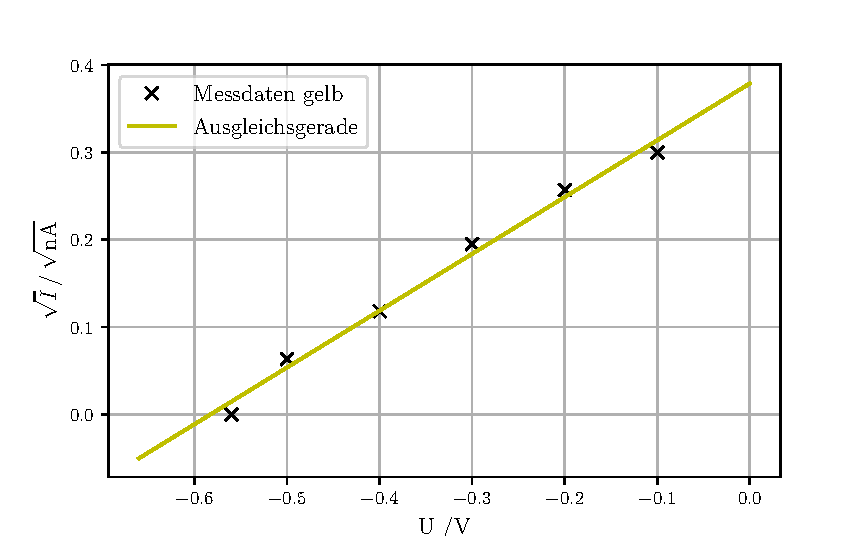
\includegraphics[width=\textwidth]{build/plot1b.pdf}
  \caption{Messwerte der Gegenfeldmethode für das gelbes Licht mit der Ausgleichsgerade.}
  \label{fig:plot1b}
\end{figure}
\begin{table}[H]
  \centering
  \caption{Messwerte für das gelbe Licht.}
  \label{tab:gelb}
  \sisetup{table-format=2.2}
  \begin{tabular}{S S[table-format=1.3] }
  \toprule
  {Spannung $U / \si{\volt}$} & {Stromstärke $ I / \si{\nano\ampere}$}\\
  \midrule
  -0.56 &  0     \\
  -0.50 &  0.004 \\
  -0.40 &  0.014 \\
  -0.30 &  0.038 \\
  -0.20 &  0.066 \\
  -0.10 &  0.090 \\
  -0.02 &  0.100 \\
   0.02 &  0.120 \\
   0.10 &  0.125 \\
   0.20 &  0.130 \\
   0.30 &  0.150 \\
   0.40 &  0.160 \\
   0.50 &  0.200 \\
   1.00 &  0.420 \\
   1.50 &  0.500 \\
   2.00 &  0.560 \\
   2.50 &  0.580 \\
   3.00 &  0.650 \\
   3.50 &  0.550 \\
   4.00 &  0.600 \\
   4.50 &  0.800 \\
   5.00 &  0.700 \\
   6.00 &  0.700 \\
   7.00 &  0.750 \\
   8.00 &  0.750 \\
   9.00 &  0.800 \\
  10.00 &  0.850 \\
  12.50 &  0.900 \\
  15.00 &  0.950 \\
  17.50 &  1.000 \\
  19.00 &  1.600 \\
  \bottomrule
  \end{tabular}
\end{table}
Die bestimmten Werte für das grüne Licht werde in \autoref{tab:grün} eingetragen. 
In \autoref{fig:plot2} wird die Wurzel der Stromstärke gegenüber der der Spannung für grünes Licht eingetragen.
Auch hier wird eine Ausgleichsgerade eingefügt und die Parameter werden in \autoref{tab:Frequenzen} eingetragen.
\begin{table}[H]
  \centering
  \caption{Messwerte für das grüne Licht.}
  \label{tab:grün}
  \sisetup{table-format=2.2}
  \begin{tabular}{S S[table-format=1.3] }
  \toprule
  {Spannung $U / \si{\volt}$} & {Stromstärke $ I / \si{\nano\ampere}$}\\
  \midrule
  -0.02 &  0.310 \\
  -0.10 &  0.280 \\
  -0.20 &  0.220 \\
  -0.30 &  0.200 \\
  -0.40 &  0.090 \\
  -0.45 &  0.050 \\
  -0.50 &  0.048 \\
  -0.55 &  0.020 \\
  -0.60 &  0.010 \\
  -0.65 &  0.004 \\
  -0.70 &  0     \\
  \bottomrule
  \end{tabular}
\end{table}
\begin{figure}[H]
  \centering
  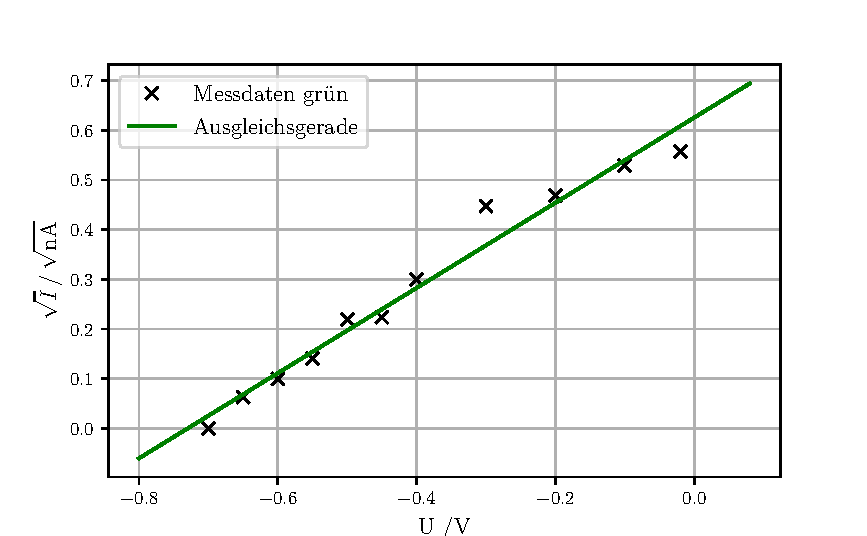
\includegraphics[width=\textwidth]{build/plot2.pdf}
  \caption{Messwerte der Gegenfeldmethode für das grüne Licht mit der Ausgleichsgerade.}
  \label{fig:plot2}
\end{figure}
In \autoref{tab:türkis} werden die Messwerte für das türkise Licht eingetragen und in \autoref{fig:plot3} dargestellt.
Dabei wird die Wurzel der Stromstärke gegenüber der Spannung gestellt.
Die Ausgleichsgerade wird auch eingetragen und die Parameter sind in \autoref{tab:Frequenzen} eingefügt.
\begin{table}[H]
  \centering
  \caption{Messwerte für das türkise Licht.}
  \label{tab:türkis}
  \sisetup{table-format=2.2}
  \begin{tabular}{S S[table-format=1.3] }
  \toprule
  {Spannung $U / \si{\volt}$} & {Stromstärke $ I / \si{\nano\ampere}$}\\
  \midrule
  -0.02 &  0.030 \\
  -0.10 &  0.022 \\
  -0.20 &  0.020 \\
  -0.30 &  0.018 \\
  -0.40 &  0.016 \\
  -0.50 &  0.010 \\
  -0.60 &  0.008 \\
  -0.70 &  0.004 \\
  -0.80 &  0.001 \\
  -0.90 &  0     \\
  \bottomrule
  \end{tabular}
\end{table}
\begin{figure}[H]
  \centering
  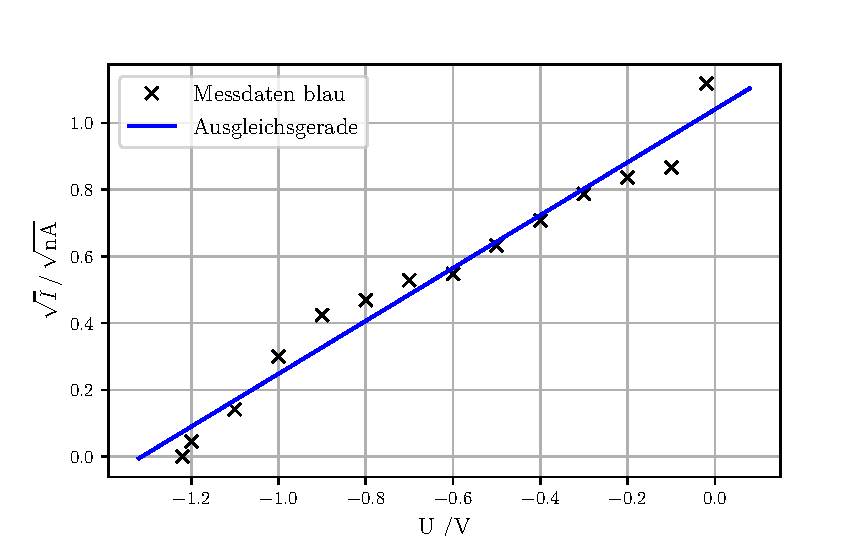
\includegraphics[width=\textwidth]{build/plot3.pdf}
  \caption{Messwerte für das türkise Licht mit der Ausgleichsgerade.}
  \label{fig:plot3}
\end{figure}
Die Werte der Messung für das blaue Licht sind in \autoref{tab:blau} eingetragen und in \autoref{fig:plot4} dargestellt mit einer Ausgleichgerade.
Die Wurzel der Stromstärke wird dabei gegenüber der Spannung aufgetragen.
\begin{figure}[H]
  \centering
  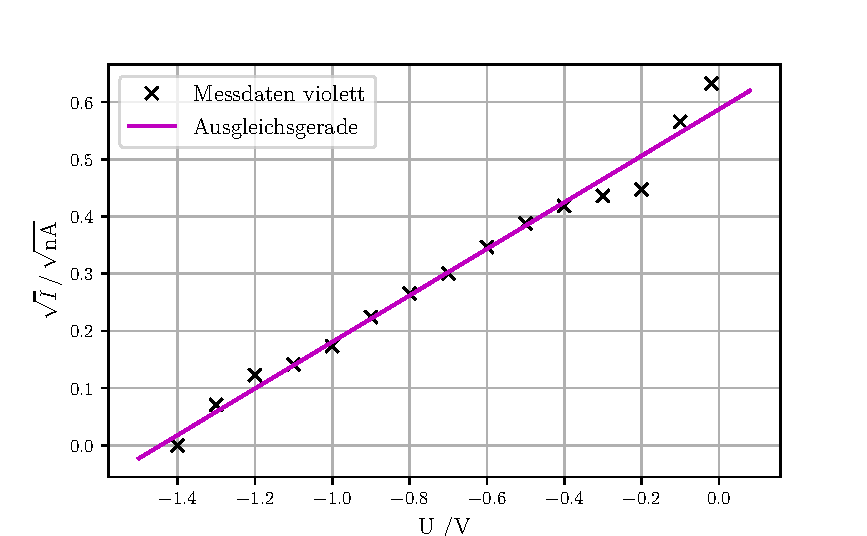
\includegraphics[width=\textwidth]{build/plot4.pdf}
  \caption{Messwerte für das blaue Licht mit der Ausgleichsgerade.}
  \label{fig:plot4}
\end{figure}
\begin{table}[H]
  \centering
  \caption{Messwerte für das blaue Licht.}
  \label{tab:blau}
  \sisetup{table-format=2.2}
  \begin{tabular}{S S[table-format=1.3] }
  \toprule
  {Spannung $U / \si{\volt}$} & {Stromstärke $ I / \si{\nano\ampere}$}\\
  \midrule
  -0.02 &  1.250 \\
  -0.10 &  0.750 \\
  -0.20 &  0.700 \\
  -0.30 &  0.620 \\
  -0.40 &  0.500 \\
  -0.50 &  0.400 \\
  -0.60 &  0.300 \\
  -0.70 &  0.280 \\
  -0.80 &  0.220 \\
  -0.90 &  0.180 \\
  -1.00 &  0.090 \\
  -1.10 &  0.020 \\
  -1.20 &  0.002 \\
  -1.22 &  0     \\
  \bottomrule
  \end{tabular}
\end{table}
Das violette Licht wird gemessen und und in \autoref{tab:violett} eingetragen. Die Wurzel der Stromstärke wird gegenüber der Spannung in
\autoref{fig:plot5} eingetragen mit einer Ausgleichsgerade. Die berechneten Parameter der Ausgleichgerade werden in \autoref{tab:Frequenzen}
eingetragen.
\begin{table}[H]
  \centering
  \caption{Messwerte für das violette Licht.}
  \label{tab:violett}
  \sisetup{table-format=2.2}
  \begin{tabular}{S S[table-format=1.3] }
  \toprule
  {Spannung $U / \si{\volt}$} & {Stromstärke $ I / \si{\nano\ampere}$}\\
  \midrule
  -0.02 &  0.400 \\
  -0.10 &  0.320 \\
  -0.20 &  0.200 \\
  -0.30 &  0.190 \\
  -0.40 &  0.175 \\
  -0.50 &  0.150 \\
  -0.60 &  0.120 \\
  -0.70 &  0.090 \\
  -0.80 &  0.070 \\
  -0.90 &  0.050 \\
  -1.00 &  0.030 \\
  -1.10 &  0.020 \\
  -1.20 &  0.015 \\
  -1.30 &  0.005 \\
  -1.40 &  0     \\
  \bottomrule
  \end{tabular}
\end{table}
\begin{figure}[H]
  \centering
  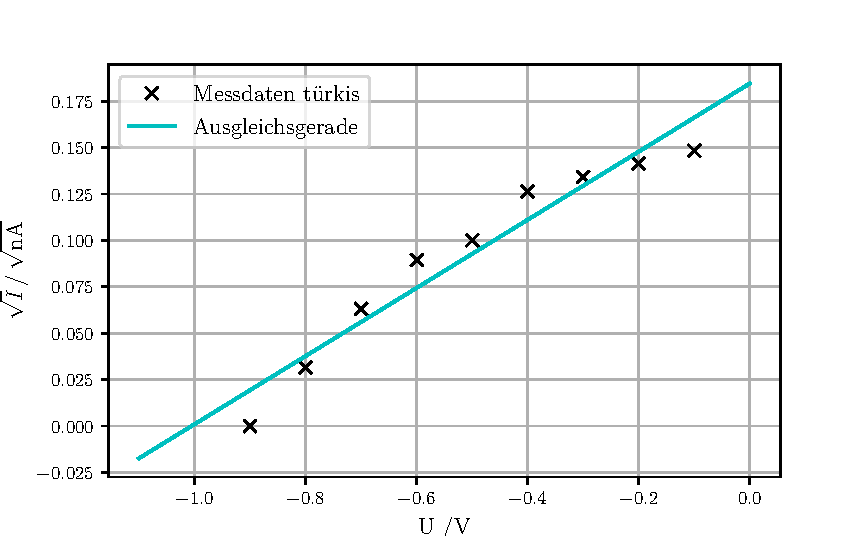
\includegraphics[width=\textwidth]{build/plot5.pdf}
  \caption{Messwerte für das violette Licht mit der Ausgleichsgerade.}
  \label{fig:plot5}
\end{figure}
%ende von Grebzfrequenz
\subsection{Bestimmung von $\frac{h}{e}$ und der Austrittsarbeit} % (fold)
\label{sub:Austrittsarbeit}


Aus den gegebenen Wellenlängen(\cite[80]{V500}) werden die Frequenzen für verschiedene Farben berechnet mit \autoref{eqn:Frequenz}
und in \autoref{tab:Frequenzen} eingetragen.
Mithilfe der Parameter der Ausgleichsgeraden wird mit
\begin{align*}
  U_g = - \frac{b}{a}
\end{align*}
die Grenzspannung berechnet und auch in \autoref{tab:Frequenzen} eingetragen.
\begin{table}[H]
  \centering
  \caption{Berechnete Frequenzen und Parameter der Ausgleichsgeraden für verschiedene Farben.}
  \label{tab:Frequenzen}
  \sisetup{table-format=1.3}
  \begin{tabular}{c S[table-format=3.0] S[table-format=3.2] S@{${}\pm{}$} S S@{${}\pm{}$} S S[table-format=3.3]@{${}\pm{}$} S }
  \toprule
  {Farbe} & {$\lambda / \si{\nano\metre}$} & {$\nu / \si{\tera\hertz}$} &\multicolumn{2}{c}{$a / \sqrt{\si{\nano\ampere}} / \si{\volt}$} & \multicolumn{2}{c}{$b / \sqrt{\si{\nano\ampere}}$} & \multicolumn{2}{c}{$ U_g / \si{\volt}$} \\
  \midrule
    gelb    & 578 & 518.67 & 0.650 & 0.033 & 0.379 & 0.013 & -0.583 & 0.035 \\
    grün    & 546 & 549.07 & 0.857 & 0.049 & 0.625 & 0.023 & -0.730 & 0.050 \\
    türkis  & 492 & 609.33 & 0.184 & 0.018 & 0.185 & 0.010 & -1.005 & 0.113 \\
    blau    & 435 & 689.18 & 0.792 & 0.043 & 1.040 & 0.032 & -1.313 & 0.082 \\
    violett & 408 & 734.79 & 0.407 & 0.155 & 0.587 & 0.013 & -1.444 & 0.063 \\
  \bottomrule
  \end{tabular}
\end{table}

Die ermittelten Werte der Grenzspannungen werden gegen die jeweilige Frequenz aufgetragen.
Das Ergebnis ist in \autoref{fig:plot7} dargestellt.
Außerdem wird eine Ausgleichsgerade erstellt.
\begin{figure}[H]
  \centering
  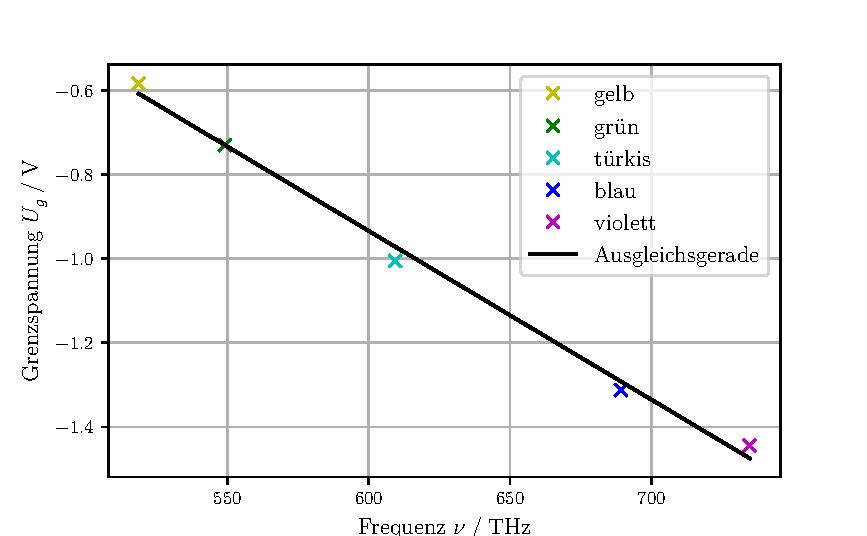
\includegraphics[width=\textwidth]{plot7.pdf}
  \caption{Grenzspannungen aufgetragen gegenüber der Frequenz.}
  \label{fig:plot7}
\end{figure}

Mithilfe der Parameter der Ausgleichsgerade
\begin{align*}
  a &= (-4.014 \pm 0.177) 10^4 \si{\volt\second} \\
  b &= (1.474 \pm 0.111) \si{\volt}
\end{align*}
wird das Verhältnis von $h$ und $e$, sowie die Austrittsarbeit bestimmt zu
\begin{align*}
  \frac{h}{e} &= (4.014 \pm 0.177) 10^4 \si{\volt\second} \\
  A_K &=  (1.474 \pm 0.111) \si{\electronvolt}.
\end{align*}

%ende von Austrittsarbeit

\subsection{Nähere Betrachtung des Photostroms vom gelben Licht} % (fold)
\label{sub:Nähere Betrachtung des Photostroms vom gelben Licht}

\begin{figure}[H]
  \centering
  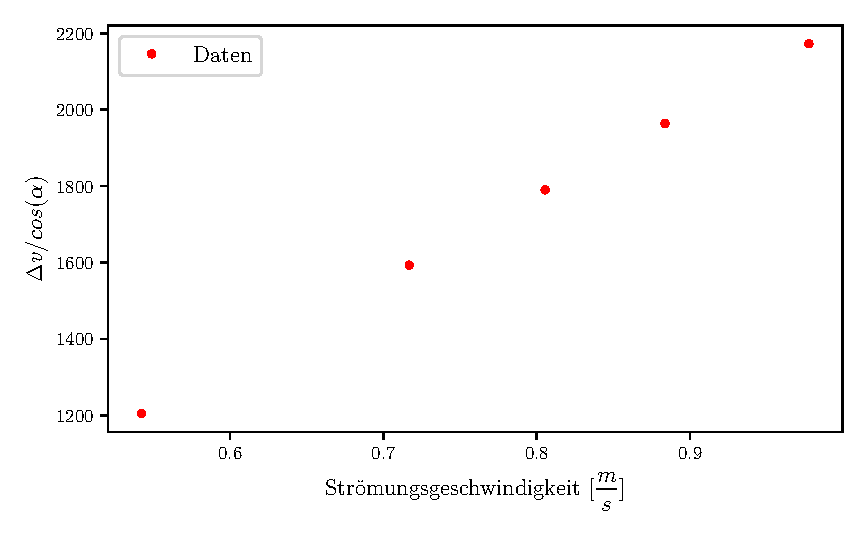
\includegraphics[width=\textwidth]{plot1.pdf}
  \caption{Photostrom für gelbes Licht aufgetragen gegen die Spannung.}
  \label{fig:plot1}
\end{figure}

Die Kurve erreicht bei hohen Spannungen einen Sättigungswert, bzw. nähert sich asymptotisch einem Grenzwert an.
Da die Anzahl der emittierten Elektronen von der endlichen Intensität der eingestrahlten Lichtstrahlung abhängig ist,
nähert sie sich bei konstanter Lichtstrahlung einem endlichen Wert an.
Die kinetische Energie der Elektronen ist ungleich verteilt, daher können manche Elektronen die Anode verfehlen,
weil diese zusätzlich eine endliche Größe besitzt. Somit müsste die Anode vergrößert werden und der Glaszylinder muss perfekt
evakuiert werden, um eine Photozelle zu konstruieren, wo der Sättigungswert nicht nur asymptotisch erreicht wird.\\
Die Elektronen haben aufgrund der Fermi-Dirac-Verteilung in der Photokathode bereits unterschiedliche Energien.
Dies führt dazu, dass die benötigte Energie zum herauslösen der Elektronen ebenfalls variiert.
Daher gibt es Elektronen, deren Energie trotz $U > U_G$ nicht ausreicht um die Anode zu erreichen.
Da das Kathodenmaterial schon bei Zimmertemperatur verdampft\cite{V500} und sich an der Anode absetzen kann,
kann auch hier ein photoelektrischer Effekt auftreten, der dem gewünschten Photostrom entgegen gerichtet ist.
Dieser Effekt ist recht gering gegenüber dem vorgesehnen Photoeffekt.\\
Die Anode besitzt anscheinend, da schon energiearmes Licht einen Photostromauslösen kann, eine geringe Austrittsarbeit.

% subsection Nähere Betrachtung des Photostroms vom gelben Licht (end)
